\section{Application Security Basics}

\subsection{HTTP Basics}

HTTP ist \textbf{Zustandslos}: Der Client sendet eine Anfrage (\textbf{Request}) an den Server, welcher ihn verarbeitet und anschliessend das Resultat als Antwort (\textbf{Response}) zurücksendet.\\

\begin{figure}[H]
	\centering
	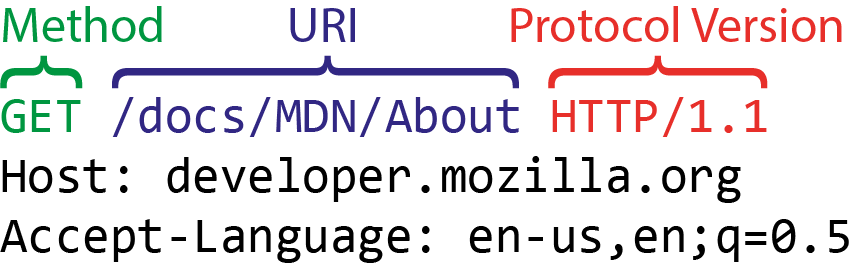
\includegraphics[width=0.38\textwidth]{./img/http-head}
	\caption{HTTP Header}
\end{figure}

Zwischen HTTP GET und POST gibt es einen wesentlichen Unterschied. Da der Server die URI in der Regel mitloggt, werden auch die \textbf{Parameter des GET-Request mitgeloggt}. Beim POST-Request geschieht dies nicht, da sich die Parameter anstatt in der URI im Body befinden. Dies ist auch bei Proxies zu beachten. Eine \textbf{Response} ist beinahe Identisch zum Request. Die erste Zeile enthält nun das Protokoll, Statuscode und Statusbeschreibung (HTTP/1.1 200 OK).

\begin{figure}[H]
	\centering
	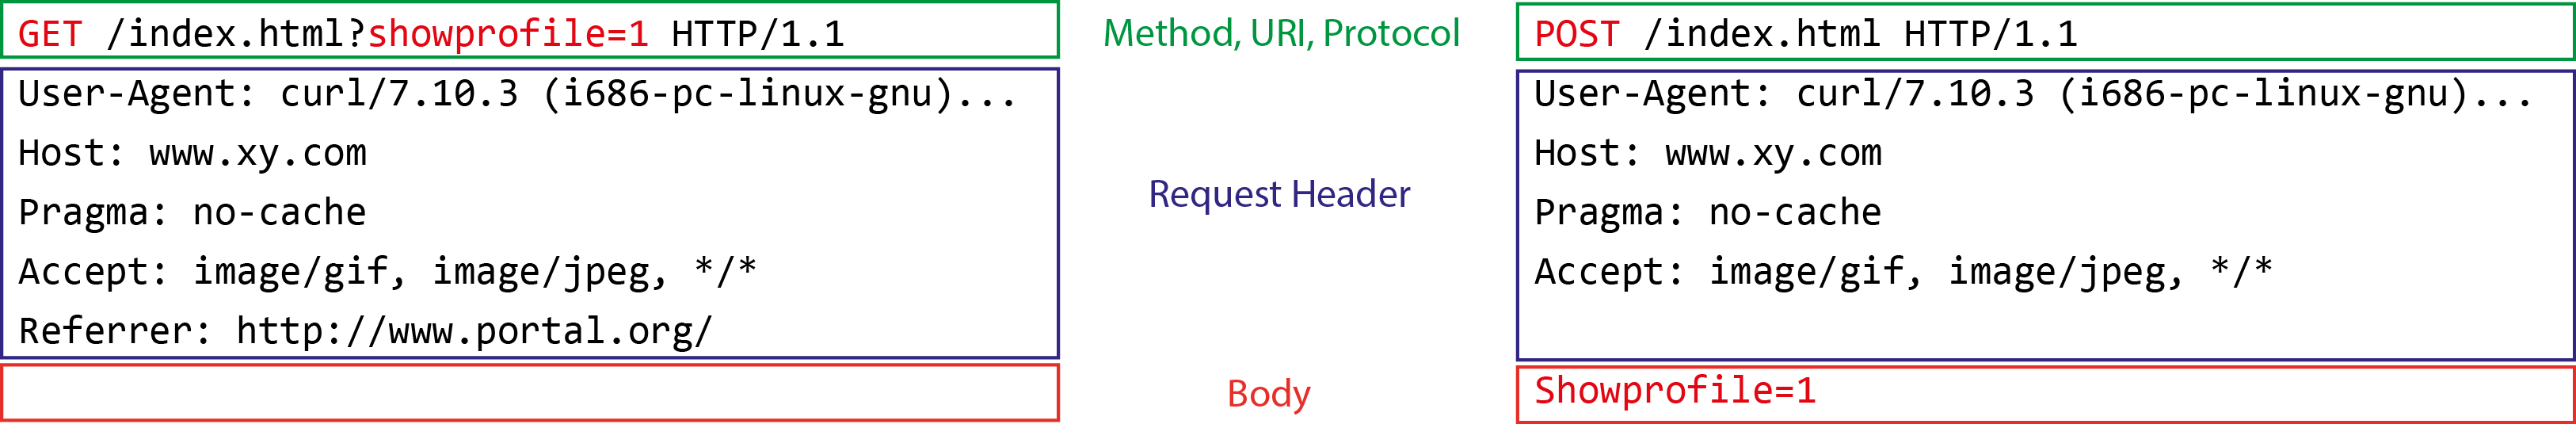
\includegraphics[width=\textwidth]{./img/http-full-request}
	\caption{Beispielrequests für GET und POST}
\end{figure}

\begin{table}[H]
	\begin{tabularx}{\textwidth}{l|X}
		\textbf{HTTP Methode} & \textbf{Verwendung}\\ \hline
		GET		& normale verwendung *\\ \hline
		POST	& übermittlung von Daten (Login, Formulare) *\\ \hline
		HEAD	& Suchmaschinen (Head of page) *\\ \hline
		PUT		& Upload von Dateien (webdav, RESTful)\\ \hline
		DELETE	& Löschen von Dateien (webdav, RESTful)\\ \hline
		OPTIONS	& Auflistung verfügbarer Methoden auf Server\\ \hline
		TRACE	& Debugging in Webserver\\ \hline
	\end{tabularx}
	\caption{Übliche HTTP Methoden (* meist verwendet)}
\end{table}


\begin{table}[H]
	\begin{tabularx}{\textwidth}{l|p{100pt}|X}
		\textbf{Statuscode} & \textbf{Nachricht} & \textbf{Bedeutung}\\ \hline
		\multicolumn{3}{c}{2xx - Erfolgreich} \\ \hline
		200 & OK & Anfrage erfolgreich bearbeitet, Ergebnis in der Antwort enthalten. \\ \hline
		\multicolumn{3}{c}{3xx - Umleitung} \\ \hline
		301 & Moved Permanently & Header "'Location: http://other-site/"' \\ \hline
		302 & Moved Temporarily & Header "'Location: http://other-site/"'; Alternativ 303 oder 307 möglich \\ \hline
		\multicolumn{3}{c}{4xx - Clientfehler} \\ \hline
		400 & Bad Request & Anfrage war fehlerhaft aufgebaut \\ \hline
		401 & Unauthorized & Authentifizierung nötig \\ \hline
		403 & Forbidden & Mangelnde Berechtigung des Clients \\ \hline
		404 & Not Found & Angeforderte Ressource nicht gefunden \\ \hline
		405 & Method Not Allowed & \\ \hline
		408 & Request Timeout & \\ \hline
		\multicolumn{3}{c}{5xx - Serverfehler} \\ \hline
		500 & Internal Server Error & Allgemeiner Serverfehler \\ \hline
		501 & Not Implemented & Funktionalität wird vom Server nicht bereitgestellt \\ \hline
		502 & Bad Gateway & Proxy hat ungültige Antwort erhalten \\ \hline
		503 & Service Unavailable & Service steht temporär nicht zur verfügung \\ \hline
	\end{tabularx}
	\caption{Übliche HTTP Statuscodes, \url{https://de.wikipedia.org/wiki/HTTP-Statuscode}}
\end{table}

\subsection{Redirect after succesful login}
Unter diesem Namen verbirgt sich ein Pattern, um die "'\textbf{Back Button Relogin Vulnerability}"' zu adressieren. Ohne Anwendung dieses Patterns besteht die Möglichkeit, dass nach mehrmaligem Klick auf Zurück die eingegebenen Logindaten erneut an den Server übertragen werden. Bei Fehlschlag des Logins kann mittels eines gewöhnlichen \textit{200 OK} um eine erneute Eingabe gebeten werden.

\begin{figure}[H]
	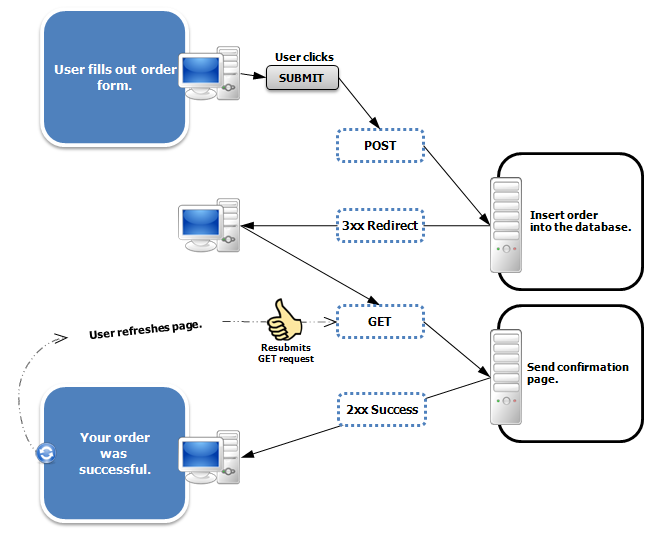
\includegraphics[width=\textwidth]{./img/PostRedirectGet_DoubleSubmitSolution}
	\caption{Redirect after succesful login}
\end{figure}

Es gibt dabei mehrere Varianten für den Redirect:
\begin{easylist}
	& Type 1 (302 Moved Temporarily)
	&& HTTP Response Status 302
	&& HTTP Response Header "'Location: http://other-site/"'
	& Type 2 (200 OK)
	&& HTTP Response Status 200
	&& HTTP Response Header "'Refresh: 0; URL=http://other-site/"'
	& Type 3 (200 OK)
	&& HTTP Response Page
	&& Meta-Tag "'Refresh"'
	& Type 4 (Javascript)
	&& Client-Seitiger Code (z.B. "'document.location=\ldots"')
\end{easylist}

\subsection{HTTP Session Management}
Serverseitig wird eine Speicherstruktur erstellt, um Session-Daten zu speichern. Der Client erhält ein Schlüssel zu dieser Struktur, auch bekannt als \textit{SessionId}.\\
Bei jeder Anfrage des Clients an den Server muss dieser die \textit{SessionId} mitgeben, damit der Server auf die Daten der Session zugreifen kann. Dazu gibt es mehrere Varianten, wo sich die SessionId befindet (\textbf{Session Locations}):
\begin{easylist}[itemize]
	& URI
	&& Sichtbar in Logs
	&& Problematisch beim Caching
	& Request Header
	&& Cookie, NTLM, BasicAuth
	& Body
	&& Als Hidden Field
	&& Kaum verbreitet
\end{easylist}

\subsection{Cookies}

\begin{verbatim}
Set-Cookie: PREF=ID=2744d38c32b2ec68:LD=de:TM=1094031009
expires=Sun, 17-Jan-2038 19:14:07 GMT; path=/; domain=.google.ch
\end{verbatim}

\begin{figure}[H]
	\centering
	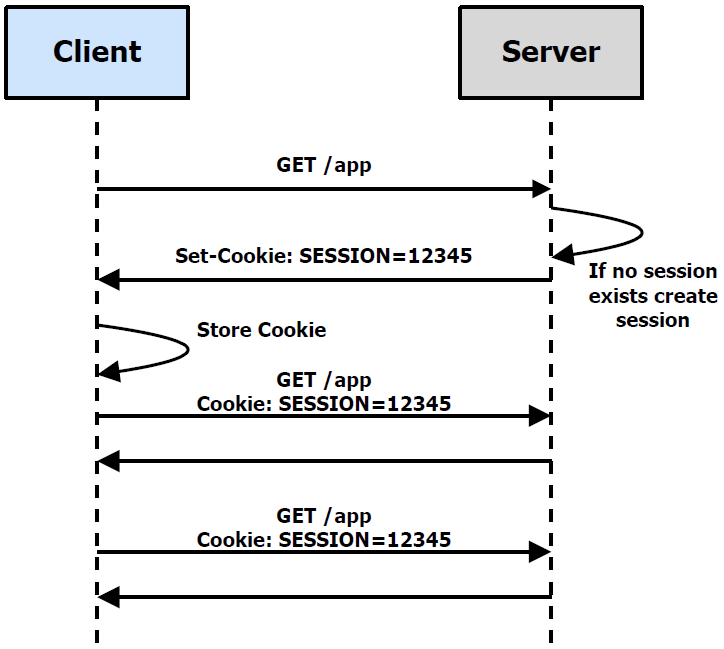
\includegraphics[width=0.6\textwidth]{./img/cookie-creation}
	\caption{Cookie erzeugung über HTTP Request Header}
\end{figure}

\subsubsection{Cookie Attribute}

\begin{easylist}[itemize]
	& \textbf{Name=Content} (Key, value pair)
	&& Name: Cookie Name
	&& Content: Cookie Value
	&& Beispiel: jsessionid=klrezbxur234kls
	& \textbf{Domain}
	&& Ort wohin das Cookie gesendet werden kann.
	&& Default: Cookie wird nur an den Server gesendet, von dem es stammt.
	& \textbf{Path}
	&& URL-Path wohin das Cookie gesendet werden kann.
	&& Default: Cookie wird nur an den Pfad gesendet, von dem es stammt.
	& \textbf{Secure}
	&& Cookie wird nur über HTTPS übermittelt.
	&& Default: insecure
	& \textbf{Expire}
	&& Gültigkeit des Cookies.
	&& Default: wird nicht persistiert, nur Browsersession.
	& \textbf{HttpOnly}
	&& Cookie kann nicht von JavaScript verwendet werden.
	&& Default: nicht vorhanden, JavaScript kann mit document.cookie darauf zugreifen.
\end{easylist}

Wann ein Cookie \textbf{an den Server gesendet} wird, ist abhängig von mehreren Attributen: Domain, Path, Secure und Expire.\\
Das HttpOnly Attribut bietet ein Schutz gegenüber XSS, wobei es dem JavaScript, welches eingeschleust wurde, verhindert wird, auf das Cookie zuzugreifen.

\subsubsection{SSL Session ID}
Mithilfe der \textit{SSL Session ID} können SSL-Session weiter verwendet werden, ohne einen erneuten Handshake durchzuführen. Ähnlich wie bei Cookies werden diese zu beginn der Anfrage an den Server übermittelt, welcher den zur ID passenden symmetrischen Schlüssel besitzt.\\
Der gesamte Payload des SSL-Pakets ist verschlüsselt, man sieht also weder die URL noch andere Inhalte des HTTP-Paket.

\subsection{Cross Site Scripting - XSS}
Die Gefahr für XSS entsteht, wenn Benutzereingaben unzureichend gefiltert werden und unverändert wieder an andere Benutzer ausgeliefert werden. Dies ermöglicht z.B. die Übernahme von Sessions, HTML- oder JS-Injection, Exploit injection oder Keylogging.\\
Es werden drei Typen von Attacken unterschieden:
\begin{description}
	\item[Stored] Das injizierte Skript ist permanent auf dem Zielserver gespeichert, z.B. in Form von Forumsbeiträgen.
	\item[Reflected] Das Skript wird nicht auf dem Zielserver gespeichert, der Angreifer muss aber eine URL präparieren und diese dem Opfer unterjubeln. Dies ist z.B. über eine Suchanfrage möglich.
	\item[DOM based] Angreifer muss eine URL präparieren, welche dann im Client direkt ausgelöst wird. Server wird dabei nicht aufgerufen, clientseitige Validierung nötig.
\end{description}

Mögliche \textbf{Gegenmassnahmen} sind:
\begin{description}
	\item[HTML entities] Encoding vor dem Speichern und bei der Ausgabe.
	\item[HTTP Only Cookies] Auslesen über JS nicht möglich.
	\item[CSP] Content Security Policy: \lstinline|script-src 'self'|
\end{description}

\subsection{Same Origin Policy}
Die damit wird verhindert, dass Javascript (auch Flash, Java Applet, etc.) auf DOM und Cookies zugreifen kann. Nur bei der Übereinstimmung von \textbf{Protokoll, Host und Port} wird dies erlaubt.\\
Wird nun aber in der Ursprungs-Seite das 3rd-Party-Script durch \lstinline|<script src="...">| geladen, so kann es auf das Cookie der Ursprungs-Seite zugreifen.\\
Die Übermittlung von Daten an fremde Seiten kann dann über Bild-Tags erfolgen, da diese nicht der SOP unterliegen.\\
Wird der Javascript-Code über die URL injiziert, so spricht man von \textbf{Reflected XSS}. Der XSS-Schutz im Browser kann dies verhindern, aber nicht bei \textbf{Stored XSS}.

\subsection{Cross Origin Resource Sharing - CORS}
Damit schützt sich nicht der eigentliche Webseitenbetreiber, sondern ein Serivce-Provider, welcher Daten für den Betreiber bereitstellt. Anfragen an den Service-Provider enthalten ein Header \lstinline|Origin: http://foo.example.com|. Die Antwort darauf den Header \lstinline|Access-Control-Allow-Origin: http://foo.example.com| (Wildcards sind auch möglich).

\subsubsection{CORS Preflighted Request}

Der Preflight wird ausgeführt, falls eine der folgenden Bedingungen zutrifft:
\begin{easylist}[itemize]
	& Verwendung einer Methode ausser GET, HEAD oder POST.
	& POST fordert Daten mit einem anderen Content-Type als \lstinline|application/x-www-form-urlencoded, multipart/form-data oder text/xml| an
	& POST sendet Daten mit einem XML-Payload zum Server.
\end{easylist}

\begin{figure}[H]
	\centering
	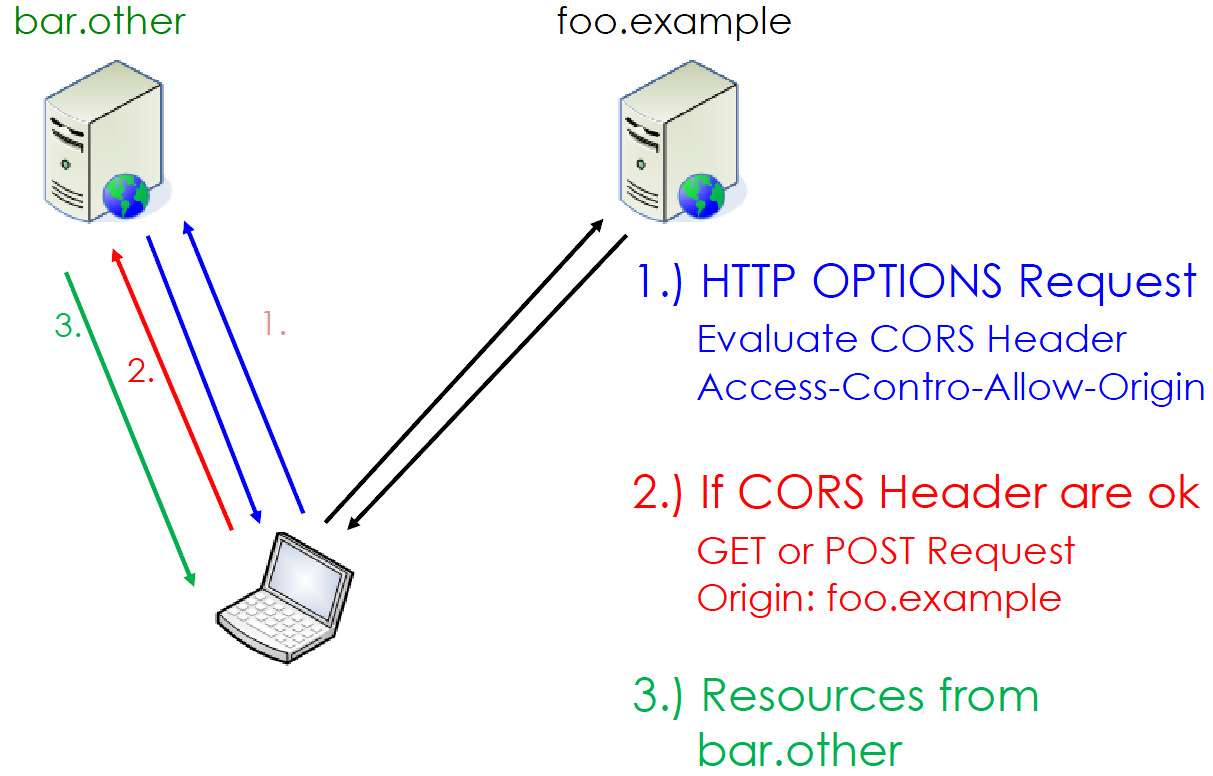
\includegraphics[width=0.6\textwidth]{./img/cors-preflight}
	\caption{Vorgehen beim CORS Preflight}
\end{figure}

Standardmässig werden bei XMLHttpRequests aufrufen keine Credentials/Cookies mitgeschickt. Um dies zu forcieren, muss ein spezielles Flag (withCredentials) auf dem Request-Objekt gesetzt werden.

\subsection{Content Security Policy - CSP}
Dahinter versteckt sich ein Sicherheitskonzept, um XSS und diverse andere Angriffe durch einschleusen von Daten in Webseiten zu verhindern. Es wird als HTTP-Header-Field \textit{Content-Security-Policy} und bei IE 10+ \textit{X-Content-Security-Policy} unterstützt.

\begin{lstlisting}[caption=Starter Policy für CSP-Header, language={}]
Content-Security-Policy: default-src 'none'; script-src 'self'; connect-src 'self'; img-src 'self'; style-src 'self';
\end{lstlisting}

Das Vorgehen beim erstellen einer neuen CSP ist wie folgt:
\begin{enumerate}
	\item CSP-Header bei allen Requests hinzufügen mit Policy \lstinline[language=clean]|default-src 'none'|
	\item Verstösse in der Browser-Konsole anschauen
	\item Nötige Quellen zur Policy hinzufügen
\end{enumerate}

\subsection{X-Frame-Headers}
Als HTTP-Header-Feld eingesetzt dient es als Schutz vor \textbf{Clickjacking}-Attacken. Dabei wird dem Opfer ein Frame über ein anderen Inhalt gelegt und so versucht, durch Klicken Aktionen auf dem dahinterliegenden Objekt auszuführen.\\
\textbf{CSP hat Vorrang} vor X-Frame-Headers, weil die Unterbindung von Frames seit Version 2.0 dort auch integriert ist.

\begin{lstlisting}[caption=Clickjacking mittels X-Frame-Options unterbinden, language={}]
X-Frame-Options: DENY
\end{lstlisting}

\subsection{HTTP Strict Transport Security - HSTS}
Ein Sicherheitsmechanismus für HTTPS-Verbindungen. Er soll vor Aushebelung der Verbindungsverschlüsselung durch eine Downgrade-Attacke als auch vor Session Hijacking schützen. Durch die Angabe des Header-Feldes wird jede weitere Verbindung bis zum erreichen des \textit{max-age} als \textbf{HTTPS erzwungen}, auch wenn die Links z.B. auf HTTP lauten. Zusätzlich wird eine Verbindung mit dem Server verhindert, sobald \textbf{Zertifikatsprobleme} auftauchen.\\

Google Chrome wie auch andere Browser verwenden \textbf{HSTS-Preload-Listen}. Damit wird die Limitierung des \textit{trust on first use}-Prinzip für eine definierte Liste von Domains umgangen.

\begin{lstlisting}[language={},caption=HSTS-Header]
Strict-Transport-Security: max-age=31536000
\end{lstlisting}

\subsection{X-XSS-Protection}
Dieser Header aktiviert den XSS-Schutz im Browser, jedoch kann dieser nur Reflected XSS erkennen. Bisher wird es nur von IE, Chrome und Safari unterstützt. In diesen Browser sollte er jedoch standardmässig bereits aktiviert sein.

\begin{lstlisting}[language={},caption=Beispiel des X-XSS-Protection Headers]
X-XSS-Protection: 1; mode=block
\end{lstlisting}

\subsection{HTTP Public Key Pinning - HPKP}
Eine Erweiterung für HTTP, das dem Webclient mitteilt, einen spezifischen kryptographischen Schlüssel mit einem bestimmten Webserver in Verbindung zu bringen. So sollen Man-in-the-Middle-Angriffe mit gefälschten Zertifikaten vermieden werden.\\

Google Chrome wie auch Firefox verwenden \textbf{Preload-Listen}. Damit wird die Limitierung des \textit{trust on first use}-Prinzip für eine definierte Liste von Domains umgangen.

\begin{lstlisting}[language={},caption=Beispiel des HPKP-Headers]
Public-Key-Pins: pin-sha256="base64=="; max-age=expireTime [; includeSubdomains][; report-uri="reportURI"]
\end{lstlisting}